\section{Spezifikation der Anforderungen}
Im nun folgenden Unterkapitel werden die im letzten Kapitel, durch Onlinebefragung und in persönlichen Gesprächen, ermittelten Anforderungen spezifiziert, das heißt, systematisch ausgewertet. Es wird aufgrund einer nichtvorhandenen Ausschreibung des Projekts und des geringen Projektumfangs auf ein seperates Lasten- und Pflichtenheft verzichtet und stattdessen die Anforderungen in der hier beginnenden \glqq{}Requirements Specification\grqq{}, zu deutsch \glqq{}Anforderungsspezifikation\grqq{}, niedergeschrieben. Dazu wird sich an der von Helmut Balzert beschriebenen \glqq{}Schablone[n] für Lastenheft, Pflichtenheft und Glossar\grqq{}\footcite[S. 492]{balzert} orientiert. In dieser werden zuerst die Visionen und Ziele des Entwicklungsprojekt verfasst, danach die Rahmenbedingungen denen die Entwicklung unterliegt, im Anschluss der technische Kontext, in dem sich die Entwicklung abspielt und dann erst die funktionalen Anforderungen, die die Kernfunktionalität des Systems beschreiben gefolgt von den nichtfunktionalen Anforderungen, bzw. den Qualitätsanforderungen, in denen die messbare Qualität und das Verhalten des Systems beschrieben wird.\footcite[Vgl.][S. 492 ff.]{balzert}. Die Anforderungen sind natursprachlich verfasst und verfügen über einen einzigartigen Identifikator, um im späteren Verlauf auf sie verweisen zu können. Diese sind so aufgebaut, dass \glqq{} [j]ede Anforderung [..] mit einem Buchstaben [beginnt] [...], gefolgt von einer Zahl, eingschlossen in Schrägstriche. Der Anforderungstyp wird durch einen Buchstaben gekennzeichnet [...].\grqq{} \footcite[S. 493]{balzert}

\subsection{Visionen und Ziele}
Die hier aufgezählten Visionen und Ziele sind Ausdruck der mit dem fertigen Produkt zu erreichenden Zukunft. Visionen sind dabei abstrakter und generisch verfasst, Ziele konkretisieren diese dann im Anschluss.\footcite[Vgl.][S. 457]{balzert}
\begin{itemize}
    \item[] \emph{/V10/} Der Auftraggeber soll durch den Business Transformation Tracker eine Qualitätssteigerung und Effizienzverbesserung in seinen Transformationsprojekten erreichen.
    \item[] \emph{/V20/} Die Anwender sollen mit dem Business Transformation Tracker während des gesamten Projektzeitraums die in SAP umgesetzten Prozesse erfassen und nachverfolgen können.
    \item[] \emph{/V30/} In jedem adesso active transformation -Projekt soll der Business Transformation Tracker eingesetzt werden.
    \item[] \emph{/V40/} Das Produkt soll dem Anwender eine angenehme User Experience bieten und muss ihn in seiner Arbeit produktiv unterstützen.\\
\end{itemize}

\begin{itemize} 
    \item[] \emph{/Z10/} Der Business Transformation Tracker soll zu jedem Zeitpunkt den aktuellen Fortschritssgrad ausgeben können, um schnell eine Übersicht zu erhalten.
    \item[] \emph{/Z20/} Dem Anwender soll es möglich sein, unterschiedliche Projekt aufrufen zu können.
    \item[] \emph{/Z30/} Die Ziele der Informationssicherheit (Authentizität, Vertraulichkeit, Integrität) dürfen nicht verletzt werden.
    \item[] \emph{/Z40/} Alle bereits jetzt implementierten Funktionen werden in die Neuentwicklung übernommen.         
    \item[] \emph{/Z50/} Der Business Transformationen Tracker soll den Funktionsumfang der jetzigen Lösung überbieten.  
    \item[] \emph{/Z60/} Das Anlegen eines Projektes im BTT dauert nicht länger als eine Minute.
    \item[] \emph{/Z70/} Die Erstellung eines Prozesschrittes ist dem Benutzer intuitiv möglich.
    \item[] \emph{/Z80/} Die Anwendung ist auf den verbreitetsten Systemen, Windows, Mac und Linux, einsetzbar.
\end{itemize}

\subsection{Rahmenbedingungen}
Als Rahmenbedingungen bezeichnet man Einschränkungen, die in der Entwicklung der Software berücksichtigt werden müssen. Diese sind entweder technischer oder organisatorischer Natur.\footcite[Vgl.][S. 459 f.]{balzert}
\begin{itemize}
    \item[] \emph{/R10/}
    \item[] \emph{/R20/}
\end{itemize}

\subsection{Kontext und Überblick}
Der Kontext beschreibt die technische Umgebebung, in die die Entwicklung eingebettet ist und welche Abhängigkeiten und Schnittstellen zu anderen Systemen exisitieren.\footcite[Vgl.][S. 461 f.]{balzert} 
\begin{itemize}
    \item[] \emph{/K10/}
    \item[] \emph{/K20/}
\end{itemize}

\subsection{Funktionale Anforderungen}
Die Funktionalen Anforderungen beschreiben den Funktionsumfang des Systems. Sie werden im folgenden auf oberster Abstraktionsebene beschrieben und durch Anwendungsfälle (Use-Cases) zusammengefasst mit Hilfe von Sequenzdiagrammen und Anwendungsfalldiagrammen dargestellt.\footcite[Vgl.][S. 496]{balzert}Für die Beschreibung wird auf eine Anwendungsfallschablone zurückgegriffen, die die Eigenschaften des Anwendungsfall systematisch abfragt. Die Eigenschaften sind, das Ziel des Anwendungsfall, die Kategorie, die angibt wie häufig der Anwendungsfall ausgeführt wird, die Vorbedingung, die Nachbedingung bei Erfolg, die Nachbedingung bei Misserfolg, die Akteure des Anwendungsfall, das Auslösende Ereignis, die Beschreibung in einzelnen Schritten, die Erweiterung und mögliche Alternativen.\footcite[Vgl.][S. 261]{balzert}
\begin{figure}[h]
    \centering
    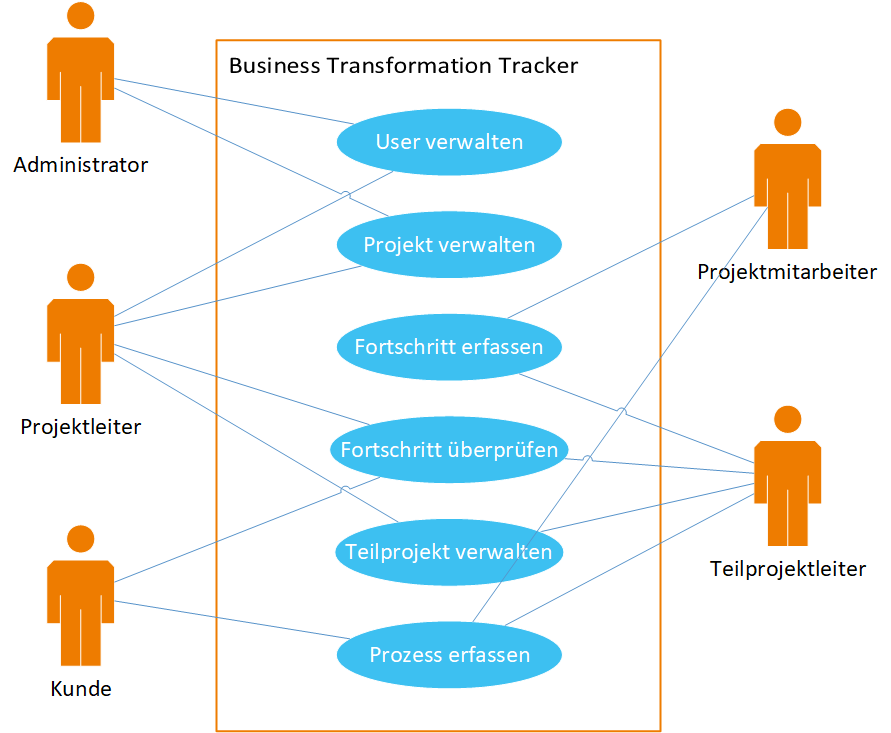
\includegraphics[scale=0.67]{./Bilder/Anwendungsfalldiagramm.png}
    \caption[Anwendungsfalldiagramm]{Anwendungsfalldiagramm mit Akteueren}
    \label{fig:Anwendungsfalldiagramm}
\end{figure}
In Abbildung \ref{fig:Anwendungsfalldiagramm} ist eine Übersicht der aus den Anforderungen erarbeiteten Anwendungsfälle zu sehen, die in den nachfolgenden Unterkapiteln anhand der oben beschriebenen Schablone genauer beschrieben werden.

\subsubsection{Anwendungsfall 1: User verwalten}
\underline{\emph{Ziel:}}\\
Es werden die für einen User hinterlegten Daten geändert. Dies kann zum einen das Passwort sein, aber auch die Stammdaten, die Rolle, oder die Zuordnung zu einem Projekt, oder Teilprojekt.\\
\underline{\emph{Kategorie:}} \\
Sekundär\\
\underline{\emph{Vorbedingung:}} \\
Der Anwender hat sich zuvor im System mit seinem Benutzernamen und Passwort angemeldet.\\
\underline{\emph{Nachbedingung Erfolg:}} \\
Die Daten und Zuordnungen des Benutzer wurden wie gewünscht angepasst.\\
\underline{\emph{Nachbedingung Fehlschlag:}} \\
Die Daten und Zuordnungen des Benutzers bleiben unverändert.\\
\underline{\emph{Akteure:}} \\
Administrator, Projektleiter\\
\underline{\emph{Auslösendes Ereignis:}} \\
Die Daten oder Zuordnungen des Benutzer müssen angepasst werden.\\
\underline{\emph{Beschreibung:}}
\begin{itemize}
    \item [1] Die Benutzerübersicht wird aufgerufen
    \item [2] Der gewünschte Benutzer wird ausgewählt.
    \item [3] Die Stammdaten des Benutzer werden editiert.
    \item [4] Die veränderten Daten werden gesichert.
\end{itemize}
\underline{\emph{Erweiterung:}}
\begin{itemize}
    \item [2a] Der Nutzer ist nicht vorhanden und wird angelegt.
    \item [3a] Der Benutzer wird einem Projekt zugeordnet.
    \item [3b] Der Benutzer wird einem Teilprojekt zugeordnet.
    \item [3c] Der Benutzer wird aus einem Projekt gelöscht.
    \item [3d] Der Benutzer wird aus einem Teilprojekt gelöscht.
    \item [3e] Das Passwort des Benutzer wird zurückgesetzt.
\end{itemize}
\underline{\emph{Alternativen:}}
\begin{itemize}
    \item [2b] Der Benutzer wird gelöscht.
    \item [3f] Die Daten sind korrekt und der Vorgang wird abgebrochen.
\end{itemize}

\subsubsection{Anwendungsfall 2: Projekt anlegen}
\underline{\emph{Ziel:}}\\
Ein neues Projekt wird hinzugefügt und die Stammdaten des Projekts werden erfasst.\\
\underline{\emph{Kategorie:}} \\
Primär\\
\underline{\emph{Vorbedingung:}} \\
Der Anwender hat sich zuvor im System mit seinem Benutzernamen und Passwort angemeldet und das Projekt ist noch nicht angelegt.\\
\underline{\emph{Nachbedingung Erfolg:}} \\
Das Projekt wird angelegt und die Stammdaten des Projekts werden wie gewünscht hinterlegt, die benötigten Projektphasen sind vorhanden und Teilprojekte sind ebenfalls angelegt.\\
\underline{\emph{Nachbedingung Fehlschlag:}} \\
Es wird kein Projekt angelegt.\\
\underline{\emph{Akteure:}} \\
Administrator, Projektleiter\\
\underline{\emph{Auslösendes Ereignis:}} \\
Es wird ein neues Projekt begonnen.\\
\underline{\emph{Beschreibung:}}
\begin{itemize}
    \item [1] Der Anwender ruft die Projektübersicht auf.
    \item [2] Ein neues Projekt wird hinzugefügt.
    \item [3] Die Stammdaten des Projekts werden hinterlegt, in Form eines Bezeichners, Beschreibung, Projektzeitraum, Kunde, und ggf. Bemerkungen.
    \item [4] Es wird ein Teilprojekt hinzugefügt.
    \item [5] Es wird eine Projektphase hinzugefügt.
    \item [6] Es werden die vorgesehenen Mitarbeiter hinzugefügt.
    \item [7] Die veränderten Daten werden gesichert.
\end{itemize}
\underline{\emph{Erweiterung:}} \\
\begin{itemize}
    \item [4a] Es werden weitere Teilprojekte hinzugefügt. 
    \item [5a] Es werden weitere Projektphasen hinzugefügt.
    \item [5b] Die Attribute der Projektphasen, die standardmäßig vorgegeben sind, werden angepasst. 
\end{itemize}
\underline{\emph{Alternativen:}} \\
./.

\subsubsection{Anwendungsfall 3: Fortschritt erfassen}
\underline{\emph{Ziel:}}\\
Der aktuell erarbeitete Fortschritt wird durch die Bearbeitung der Attribute eines Prozessschrittes dokumentiert.\\
\underline{\emph{Kategorie:}} \\
Primär\\
\underline{\emph{Vorbedingung:}} \\
Der Anwender hat sich zuvor im System mit seinem Benutzernamen und Passwort angemeldet. Es ist ein Projekt mit Teilprojekten und Projektphasen angelegt und der Bearbeiter ist dem Projekt zugeordnet.\\
\underline{\emph{Nachbedingung Erfolg:}} \\
Es wurden Projektphasenattribute in den zu bearbeitenen Prozessschritten verändert und die Fortschrittsanzeige verändert sich.\\
\underline{\emph{Nachbedingung Fehlschlag:}} \\
Es werden keine Projektphasenattribute verändert, die Fortschrittsanzeige bleibt gleich.\\
\underline{\emph{Akteure:}} \\
Teilprojektleiter, Projektmitarbeiter\\
\underline{\emph{Auslösendes Ereignis:}} \\
Außerhalb des IT-Systems wurde eine Aufgabe abgearbeitet, die anschließend dokumentiert werden muss.\\
\underline{\emph{Beschreibung:}} 
\begin{itemize}
    \item [1] Es wird die Übersicht des Projekts aufgerufen.
    \item [2] Es wird das dem Benutzer zugeordnete Teilprojekt aufgerufen.
    \item [3] Es wird der zu bearbeitene Prozess ausgewählt und innerhalb des Prozesses der entsprechende Prozessschritt.
    \item [4] Das zu ändernde Projektphasenattribut wird verändert.
    \item [5] Die Änderungen werden gespeichert.
    \item [6] Das System verändert automatisch die Fortschrittsanzeige für den entsprechenden Prozess, bzw. die Phase.
\end{itemize}

\underline{\emph{Erweiterung:}} 
\begin{itemize}
    \item [1a] Wenn der Benutzer mehreren Projekten zugeordnet ist, wechselt er zuvor in das zu bearbeitene Projekt. 
    \item [4a] Es werden weitere Projektphasenattribute verändert.
\end{itemize}
\underline{\emph{Alternativen:}}
\begin{itemize}
    \item [6a] Wenn keine Änderung stattgefunden hat, verändert sich die Fortschrittsanzeige nicht.
\end{itemize}

\subsubsection{Anwendungsfall 4: Fortschritt überprüfen}
\underline{\emph{Ziel:}}\\
Der Fortschritt in den jeweiligen Teilrojekten für die aktuelle Projektphase wird wiedergegeben.\\
\underline{\emph{Kategorie:}} \\
Sekundär\\
\underline{\emph{Vorbedingung:}} \\
Der Anwender hat sich zuvor im System mit seinem Benutzernamen und Passwort angemeldet. Es ist ein Projekt mit Teilprojekten und Projektphasen angelegt und die auswertende Person ist dem Projekt zugeordnet.\\
\underline{\emph{Nachbedingung Erfolg:}} \\
Es wird die gewünschte Auswertung ausgegeben.\\
\underline{\emph{Nachbedingung Fehlschlag:}} \\
Es wird keine Auswertung ausgegeben, wordurch der Fortschritt individuell bei den Projektmitarbeitern abgefragt werden muss.\\
\underline{\emph{Akteure:}} \\
Projektleiter, Teilprojektleiter, Kunde\\
\underline{\emph{Auslösendes Ereignis:}} \\
Während einer Überprüfung der geleisteten Arbeit soll der aktuelle Fortschritt aufgezeigt werden. Dies kann z.B. im Rahmen eines täglichen Jour Fixes geschehen.
\underline{\emph{Beschreibung:}} 
\begin{itemize}
    \item [1] Es wird die Übersicht des Projekts aufgerufen.
    \item [2] Es wird das Dashboard des Projektes aufgerufen. Dort befindet sich auf einem Blick Fortschrittsanzeigen für alle Teilprojekte in der aktuellen Projektphase.
\end{itemize}
\underline{\emph{Erweiterung:}}
\begin{itemize}
    \item [1a] Wenn der Benutzer mehreren Projekten zugeordnet ist, wechselt er zuvor in das zu bearbeitene Projekt.
\end{itemize}
\underline{\emph{Alternativen:}}
\begin{itemize}
    \item [2a] Es werden nach und nach die einzelnen Teilprojekte aufgerufen um dort eine detailliertere Aufschlüsselung des aktuellen Fortschrittes zu erhalten.
\end{itemize}

\subsubsection{Anwendungsfall 5: Teilprojekt verwalten}
\underline{\emph{Ziel:}}\\
Es werden Änderungen in einem Teilprojekt vorgenommen um die Stammdaten zu ändern, um Projektphasenattribute zu bearbeiten oder um Mitarbeiter dem Teilprojekt hinzuzufügen.\\
\underline{\emph{Kategorie:}} \\
Sekundär\\
\underline{\emph{Vorbedingung:}} \\
Es ist ein Projekt mit Teilprojekten und Projektphasen angelegt und die auswertende Person ist dem Projekt und dem zu verwaltenden Teilprojekt zugeordnet. Ein dem Teilprojekt zuzuordnener Mitarbeiter muss bereits dem Projekt zugeordnet sein.\\
\underline{\emph{Nachbedingung Erfolg:}} \\
Die Änderungen werden im System gespeichert um die Informationen im Teilprojekt werden wie gewünscht angepasst.\\
\underline{\emph{Nachbedingung Fehlschlag:}} \\
Die Änderungen werden nicht gespeichert, die Daten bleiben unverändert.\\
\underline{\emph{Akteure:}} \\
Projektleiter, Teilprojektleiter\\
\underline{\emph{Auslösendes Ereignis:}}\\
Die Daten im Teilprojekt müssen angepasst werden, weil z.B. ein neuer Mitarbeiter hinzu kommt.\\
\underline{\emph{Beschreibung:}} 
\begin{itemize}
    \item [1] Es wird die Übersicht des Projekts aufgerufen.
    \item [2] Es wird die Übersicht des Teilprojektes aufgerufen.
    \item [3] Die Stammdaten des Teilprojektes werden editiert.
\end{itemize}
\underline{\emph{Erweiterung:}}\\
./.\\
\underline{\emph{Alternativen:}}\\
\begin{itemize}
    \item [3a] Es wird ein neuer Mitarbeiter dem Teilprojekt zugeordnet.
    \item [3b] Es wird ein Projektphasenattribut hinzugefügt. 
    \item [3c] Es wird ein Projektphasenattribut entfernt.
    \item [3d] Es wird ein Projektphasenattribut verändert.
\end{itemize}

\subsubsection{Anwendungsfall 6: Prozess erfassen}
\underline{\emph{Ziel:}}\\
Die Prozesse des Kunden sind vollständig inklusive ihrer einzelen Prozessschritte im System erfasst.\\
\underline{\emph{Kategorie:}} \\
Primär\\
\underline{\emph{Vorbedingung:}} \\
Es ist ein Projekt mit Teilprojekten und Projektphasen angelegt und die auswertende Person ist dem Projekt und dem zu verwaltenden Teilprojekt zugeordnet.
\underline{\emph{Nachbedingung Erfolg:}} \\
Es sind neue Prozesse mit ihren jeweiligen Schritten im System hinterlegt.\\
\underline{\emph{Nachbedingung Fehlschlag:}} \\
Es werden keine neuen Prozesse im System erfasst.\\
\underline{\emph{Akteure:}} \\
Teilprojektleiter, Projektmitarbeiter, Kunde\\
\underline{\emph{Auslösendes Ereignis:}} \\
In einem Teilprojekt sollen zu Beginn des Projektes die Prozesse in allen Umfängen erfasst werden.\\
\underline{\emph{Beschreibung:}}
\begin{itemize}
    \item [1] Es wird die Übersicht des Projekts aufgerufen.
    \item [2] Es wird die Übersicht des Teilprojektes aufgerufen.
    \item [3] Die Prozessübersicht des Teilprojekts wird aufgerufen.
    \item [4] Es wird ein neuer Prozess angelegt.
    \item [5] Es werden die Informationen zu dem Prozess erfasst.
    \item [6] Es wird ein neuer Prozessschritt angelegt.
    \item [7] Die Änderungen werden gesichert.
\end{itemize}

\underline{\emph{Erweiterung:}}
\begin{itemize}
    \item [6a] Ein Subprozess wird erfasst.
\end{itemize}
\underline{\emph{Alternativen:}} \\
./.\\



\subsection{Qualitätsanforderungen}
Die nichtfunktionalen Anforderungen, bzw. Qualitätsanforderungen spiegeln Eigenschaften wieder, die das gesamte System und somit alle funktionalen Anforderungen betreffen. Die Qualitätsanforderungen werden anhand unterschiedlicher Kriterien kategorisiert, der \textbf{F}unktionalität, der \textbf{Z}uverlässigkeit, der \textbf{B}enutzbarkeit, der \textbf{E}ffizienz, der \textbf{W}artbarkeit und der \textbf{P}ortabilität.\footcite[Vgl.][S. 494 f.]{balzert} Die ermittelten nichtfunktionalen Anforderungen lauten wie folgt:
\begin{itemize}
    \item[] \emph{/Q10/}
    \item[] \emph{/F00/} Die Anwendung benutzt eine grafische Oberfläche.
    \vspace{0.5cm}
    \item[] \emph{/Q20/}
\end{itemize}

\begin{comment}
    Use cases
    1. Tägliches Statusupdates zur Besprechung des Fortschrittes in den Teilprojekten
    2. Anlegen eines Projektes mit seinen jeweiligen Teilprojekten und Projektphasen, Zuordnung der Rollen
    3. Initiales Erfassen eines Prozesses, mit seinen Subprozessen und den Prozessschritten
    4. Pflegen der Felder einer Projektphase 
    5. Abschließen einer Projektphase.

    Akteuere im System
    - Eigentümer des Projekts, Admin, oberes Mgmnt.
    - Projektleiter (n, normalfall 2)
    - Projektcontroller (read only)
    - Teilprojektleiter
    - Projektmitarbeiter

    \begin{itemize}
        \item[] \emph{/F10/} Die Anwendung benutzt eine grafische Oberfläche.
        
        \item[] \emph{/F20/} Es gibt unterschiedliche Benutzerrollen im System.
        
        \item[] \emph{/F30/} Die Benutzerrollen haben unterschiedliche Berechtigungen.
        \item[] \emph{/F31/} Der Benutzer loggt sich mit Benutzername und Passwort ein.
        
        \item[] \emph{/F40/} Es können ein oder mehrere Projekte angelegt und aufgerufen werden.
        
        \item[] \emph{/F50/} Ein Projekt besteht aus mehreren Projektphasen.
        \item[] \emph{/F51/} Die Projektphasen werden auf die Teilprojekte vererbt.
        
        \item[] \emph{/F60/} Innerhalb eines Projektes können ein oder mehrere Teilprojekte erstellt werden.
        
        \item[] \emph{/F70/} Innerhalb eines Projektes werden Prozesse aufgenommen
        \item[] \emph{/F80/} Die Prozesse können einem Teilprojekt zugeordnet werden oder nicht.
        \item[] \emph{/F90/} Innerhalb eines Prozesses können keine oder mehere Subprozesse aufgenommen werden.
        \item[] \emph{/F100/} Ein (Sub-)Prozess besteht aus einem oder mehreren Prozessschritten
        \item[] \emph{/F110/} Ein Prozessschritt muss einem Teilprojekt zugeordnet sein.
        \item[] \emph{/F120/}      
    \end{itemize}
    
\end{comment}
    